%---------------------------------
\section{Introduction}
\label{sec:intro}
%---------------------------------


The popularity of powerful diffusion models has led to remarkable progress in the field of content generation. For instance, text-to-image (T2I) models are capable of generating diverse and vivid images from text prompts, encompassing various visual concepts. This great success can be attributed not only to the advancement of models but also to the availability of various image data over the Internet.
Constrastingly, text-to-video (T2V) models fall short of the data categories especially in styles, since existing videos predominantly feature photorealism. While these strategies, like initializing weights from well-trained T2I models or joint training with image and video datasets, can help mitigate this issue, the generated stylized videos generally suffer from degraded style fidelity. 
% Therefore, in addition to the classic problem of \textbf{style-content decoupling} in style transfer/preserving, stylized video generation also grapples with challenges including \textbf{a scarcity of stylized video data} and the \textbf{limited capabilities of T2V base models}.
Although significant success has been achieved in style transfer/preservation in T2I generation, the field of stylized video generation remains largely unexplored,
and effective solutions are yet to be discovered.
% As one of the pioneers, AnimateDiff~\cite{guo2023animatediff} can make impressive stylized videos by combining personalized T2I models~\cite{hu2022lora} (i.e. LoRA-tuned\cite{hu2022lora} or Dreambooth-tuned\cite{dreambooth} on Stable Diffusion\cite{ldm}) with pre-trained temporal blocks. However, each style requires additional finetuning on a small set of examples, which is inefficient and unable to support any style.

% \begin{figure}[!t]
%     \centering
%     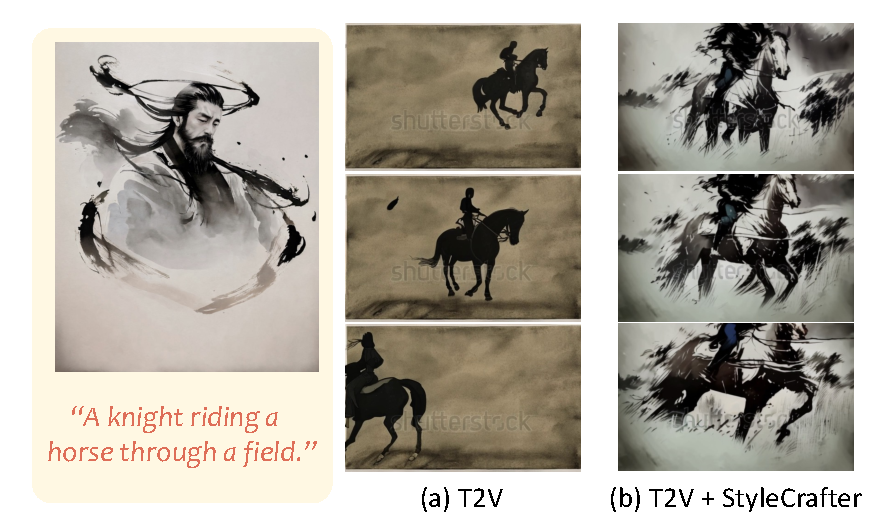
\includegraphics[width=\linewidth]{figures/motivation.pdf}\vspace{-0.5em}
%     \caption{Effect of adding style adapter to T2V models. (a) and (b) are results of Stable Diffusion~\cite{ldm} and VideoCrafter~\cite{chen2023videocrafter}. (c) is the result of VideoCrafter equipped with a style adapter. The content text prompt is "\textit{A knight riding a horse through the field}". For (a) and (b), the style prompt is generated from the style image using GPT4V~\cite{openai2023gpt4v}. \TODO{delete this figure}} 
%     \label{fig:motivation}\vspace{-0.5em}
% \end{figure}

In this paper, we propose StyleCrafter, a generic method that enhances pre-trained T2V models with a style control adapter, enabling text-to-video generation in any desired style by providing a reference image. 
% The advantages are twofold: (i) a style image offers stylistic feature guidance, complementing the stylization capabilities of T2V models in a zero-shot fashion; (ii) the reference image delivers a more accurate portrayal of the desired visual style compared to textual descriptions. 
Anyhow, it is non-trivial to achieve this goal. (i) as a classic problem of style transfer/preservation, the style control adapter requires to extract accurate style concepts from the reference image \textbf{in a content-style decoupled manner}. (ii) \textbf{the scarcity of open-source stylized videos} challenges the adaptation training of the T2V models.

Considering the scarcity of stylized videos, we propose to first train a style adapter to extract desired style concepts from images over image datasets, and then transfer the learned stylization ability to a T2V model with shared spatial weights through a tailor-made finetuning paradigm. The advantages are twofold: on the one hand, the adapter trained over stylized images can effectively extract the style concept from input images, eliminating the necessity for scarcely available stylized videos. On the other, a finetuning paradigm enables text-to-video models with better adaptation to the style concepts extracted from the previously trained style adapter, while avoiding degradation of temporal quality in video generation. 

To effectively capture the style features and promote content-style disentanglement, we adopt the widely used query transformer to extract style concepts from a single image. Particularly, we design a scale-adaptive fusion module to balance the influences of text-based content features and image-based style features, which helps generalization across various text and style combinations. During the training process, we employ carefully designed data augmentation strategies to enhance decoupled learning.

StyleCrafter efficiently generates high-quality stylized videos that align with the content of the texts and resemble the style of the reference images.
Comprehensive experiments are conducted to assess our proposed approach, demonstrating that it significantly outperforms existing competitors in both stylized image generation and stylized video generation. Furthermore, ablation studies offer a thorough analysis of the technical decisions made in developing the complete method, which provides valuable insights for the community.
Our contributions are summarized as follows:
\begin{itemize}
    \item We propose the concept of improving stylized generation for pre-trained T2V models by adding a style adapter.
    \item We explore an efficient network for stylized generation, which facilitates the content-style disentangled generation from text and image inputs. Our method attains notable advantages over existing baselines.
    \item We propose a training paradigm for generic T2V style adapter without requiring any stylized videos for supervision.
\end{itemize}